\documentclass[]{auvsi_doc}
\setkeys{auvsi_doc.cls}{
	AUVSITitle={Airframe Models},
	AUVSILogoPath={./../logo.pdf}
}

% include extra packages, if needed

\begin{document}

\begin{AUVSITitlePage}
\begin{artifacttable}
\entry{AF-011, 0.1, 02-07-2019, Initial draft, Ryan Anderson, Tyler Critchfield}
% additional \entry{} commands for extra rows in the revision table, if needed
\end{artifacttable}
\end{AUVSITitlePage}

% document contents (see below for LaTex commands that make your life easier)
\section{Introduction}
In order to predict the performance of our selected airframe, we created an aerodynamics model of the airframe using the open-source package XFLR5. This informed design decisions including CG placement and modifications to the tail in order to optimize performance. A summary of the design decisions made as a result of the XFLR5 model is included in the conclusion of this artifact for quick reference.

\section{Objective}
The objective of the XFLR5 model is to provide design guidance for the achievement of our key success measures, three of which rely significantly on the aerodynamic performance of the airframe. These include the following:
\begin{itemize}
	\item Close waypoint proximity
	\item High percentage of characteristics identified
	\item High airdrop accuracy
\end{itemize}
Each of these characteristics will be benefited by a slower stall speed than last year. Waypoint proximity and characteristics identified can be further benefited by improving static and dynamic stability, as a stable plane is easier to control and provides a more stable imaging platform for crisper images. As a system-wide requirement, the aircraft must have sufficient endurance to accomplish the above-listed objectives. With this in mind, major aerodynamic design objectives for the airframe include a slower stall speed than last year (ideally on the order of 10-15~m/s), sufficient static and dynamic stability, and a high lift-to-drag ratio to improve endurance (see Airframe Requirements Matrix). The XFLR5 model allowed us to make design decisions such as tail incidence angle and CG placement to meet these requirements.

\section{Method}
The Nimbus Pro airframe was measured, analyzed, and modeled as follows:
\subsection{Geometry}
In order to capture the aerodynamic performance of the aircraft, the wing and tail were modeled, with an extra drag term added for the fuselage. The wing, elevator, and fin were measured and modeled in the Plane Editor with geometries defined in Tables \ref{wing}, \ref{elevator}, and \ref{fin}. Airfoils were approximated by NACA foils with corresponding max camber, max camber location, and max thickness relative to the chord. These were assumed to be constant throughout the wings. Figure \ref{airfoil} shows a cross section of the wing used to determine its airfoil.

\begin{table}[H]
	\centering
	\caption{XFLR5 Wing Parameters}
	\label{wing}
	\begin{tabular}{|P{3cm}|P{4.0cm}|}
		\hline
		\rowcolor[HTML]{C0C0C0}
		{\color[HTML]{000000} \textbf{Parameter (units)}} & {\color[HTML]{000000}\textbf{Value}} \\
		\hline
		\textbf{y(m)} & [0.000 0.925 0.975] \\
		\hline
		\textbf{chord(m)} & [0.310 0.250 0.250]\\
		\hline
		\textbf{offset(m)} & [0.000 0.000 0.000] \\
		\hline
		\textbf{dihedral($^\circ)$} & [0.000 0.000 0.000] \\
		\hline
		\textbf{twist($^\circ$)} & [0.000 0.000 5.000] \\
		\hline
		\textbf{foil} & NACA 3311 \\
		\hline
	\end{tabular}
\end{table}

\begin{table}[H]
	\centering
	\caption{XFLR5 Elevator Parameters}
	\label{elevator}
	\begin{tabular}{|P{3cm}|P{4.0cm}|}
		\hline
		\rowcolor[HTML]{C0C0C0}
		{\color[HTML]{000000} \textbf{Parameter (units)}} & {\color[HTML]{000000}\textbf{Value}} \\
		\hline
		\textbf{y(m)} & [0.000 0.303] \\
		\hline
		\textbf{chord(m)} & [0.180 0.130]\\
		\hline
		\textbf{offset(m)} & [0.000 0.025] \\
		\hline
		\textbf{dihedral($^\circ)$} & [0.000 0.000] \\
		\hline
		\textbf{twist($^\circ$)} & [0.000 0.000] \\
		\hline
		\textbf{foil} & NACA 0010 \\
		\hline
	\end{tabular}
\end{table}

\begin{table}[H]
	\centering
	\caption{XFLR5 Fin Parameters}
	\label{fin}
	\begin{tabular}{|P{3cm}|P{4.0cm}|}
		\hline
		\rowcolor[HTML]{C0C0C0}
		{\color[HTML]{000000} \textbf{Parameter (units)}} & {\color[HTML]{000000}\textbf{Value}} \\
		\hline
		\textbf{y(m)} & [0.000 0.270] \\
		\hline
		\textbf{chord(m)} & [0.220 0.120]\\
		\hline
		\textbf{offset(m)} & [0.000 0.110] \\
		\hline
		\textbf{dihedral($^\circ)$} & [0.000 0.000] \\
		\hline
		\textbf{twist($^\circ$)} & [0.000 0.000] \\
		\hline
		\textbf{foil} & NACA 0010 \\
		\hline
	\end{tabular}
\end{table}

Also of note, the x location of the elevator and fin was measured to be at 0.690~m behind the wing. In order to prevent any possibility of computational singularities in the VLM solution, the elevator and fin were both placed 30~cm below the wing (i.e., z location was set to -0.300~m) as shown in Fig. \ref{locations}.

\begin{center}
	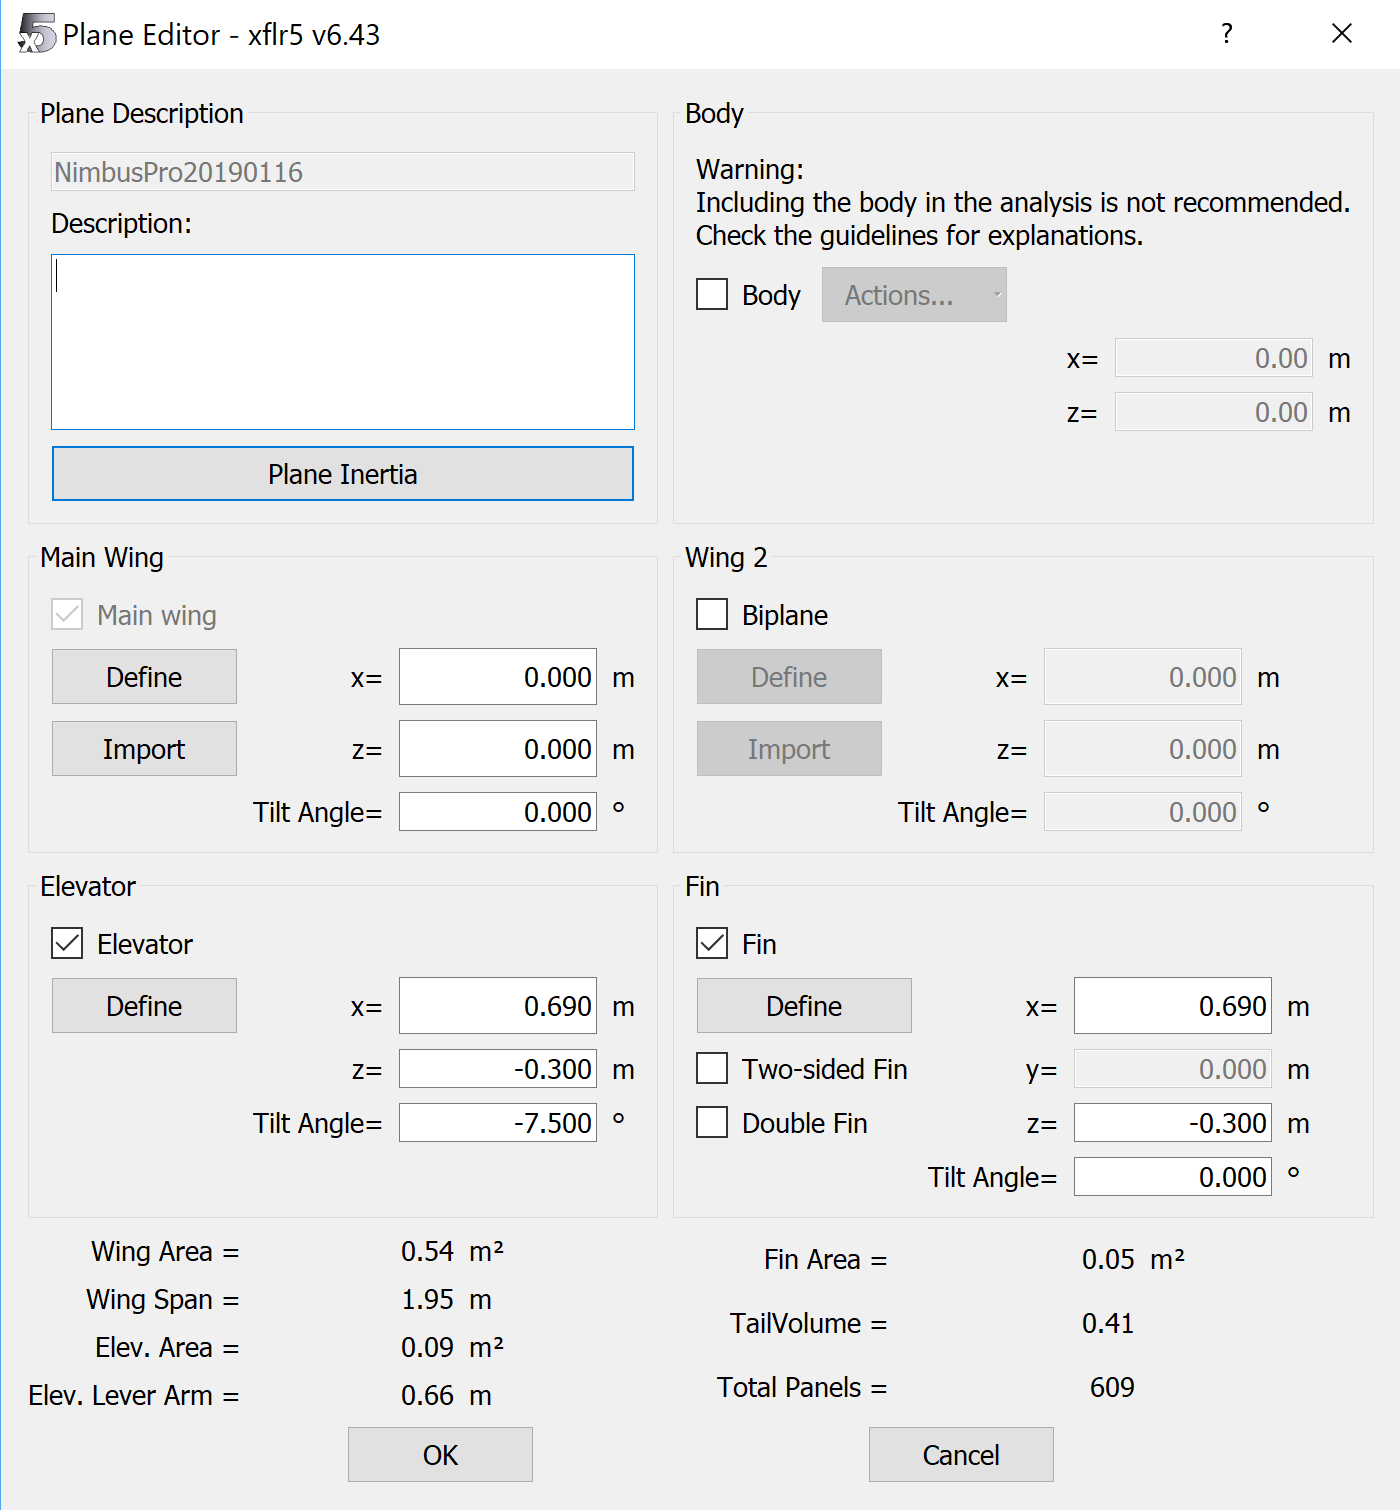
\includegraphics[width=0.80\textwidth]{./figs/wingLocations.png}
	\captionof{figure}{XFLR5 dialog summarizing wing, fin, and elevator parameters.}
	\label{locations}
\end{center}

\begin{center}
	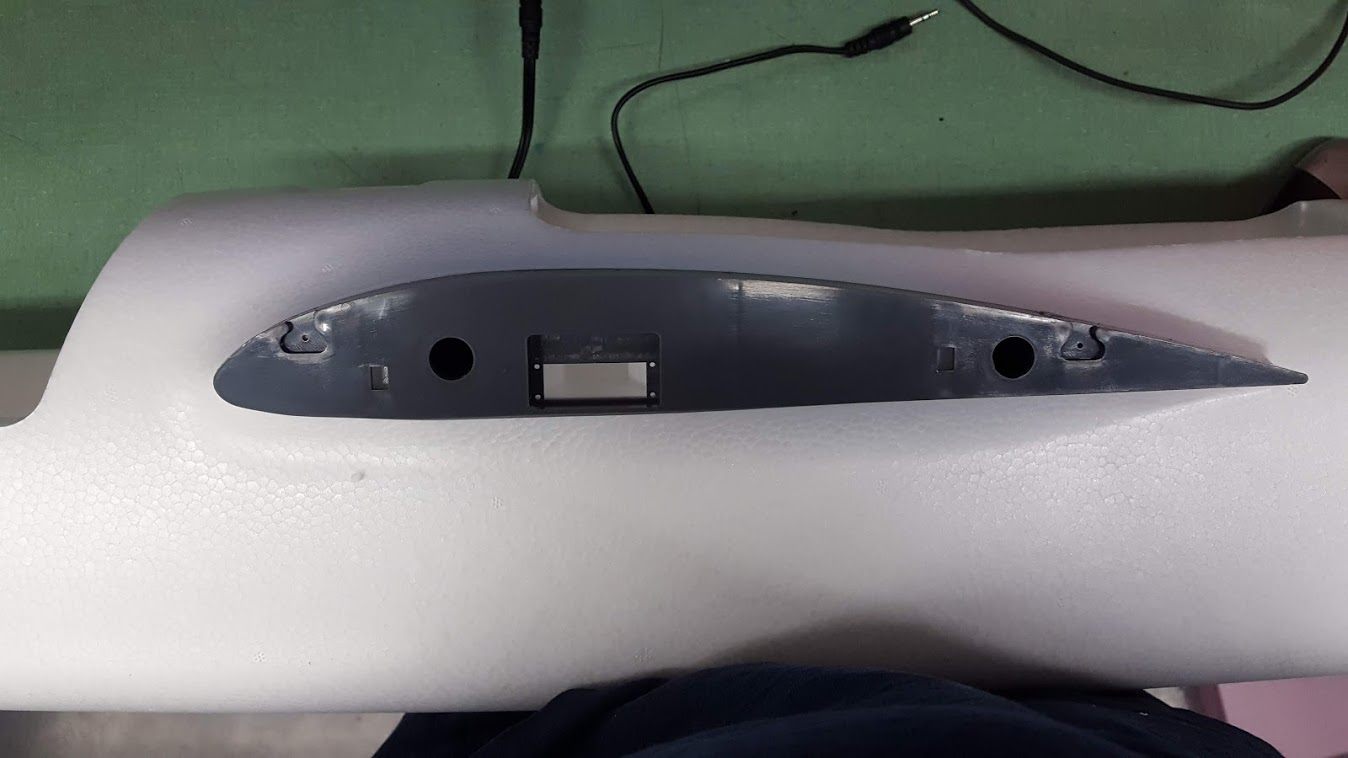
\includegraphics[width=0.95\textwidth]{./airfoils.png}
	\captionof{figure}{Cross section of the wing used to determine its airfoil.}
	\label{airfoil}
\end{center}

Finally, the weight of the airframe was determined to be 612~g, the elevator 80~g, and the fin 33~g, distributed uniformly throughout. The remainder of the plane weight was modeled as a point mass of 3095~g, in order to make the total plane weight match the measured 4.1~kg. This could be easily moved in order to change the CG location.

\subsection{Analysis}

Analyses were defined as follows.

\subsubsection{Airfoils}
First, a batch analysis was performed on the airfoils at the following conditions:
\begin{itemize}
	\item Mach = 0
	\item X transition on the upper surface (XtrTop) location: 30\%
	\item Reynold's Number list as defined in Table \ref{relist}.
	\item $\alpha$ ranging from $-8.0^\circ$ to $18.0^\circ$ at $0.25^\circ$ increments.
	\item Other parameters as shown in Fig. \ref{settings}.
\end{itemize}

\begin{center}
	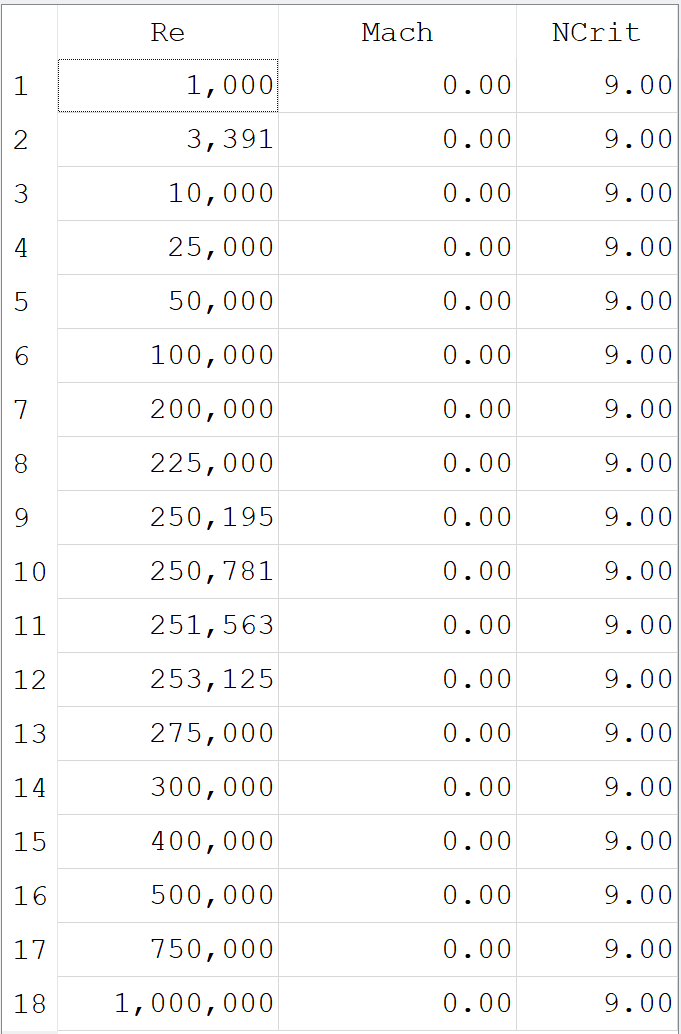
\includegraphics[width=0.35\textwidth]{./figs/airfoilAnalysisTable.png}
	\captionof{figure}{List of Reynold's Numbers used for airfoil analysis.}
	\label{relist}
\end{center}

\begin{center}
	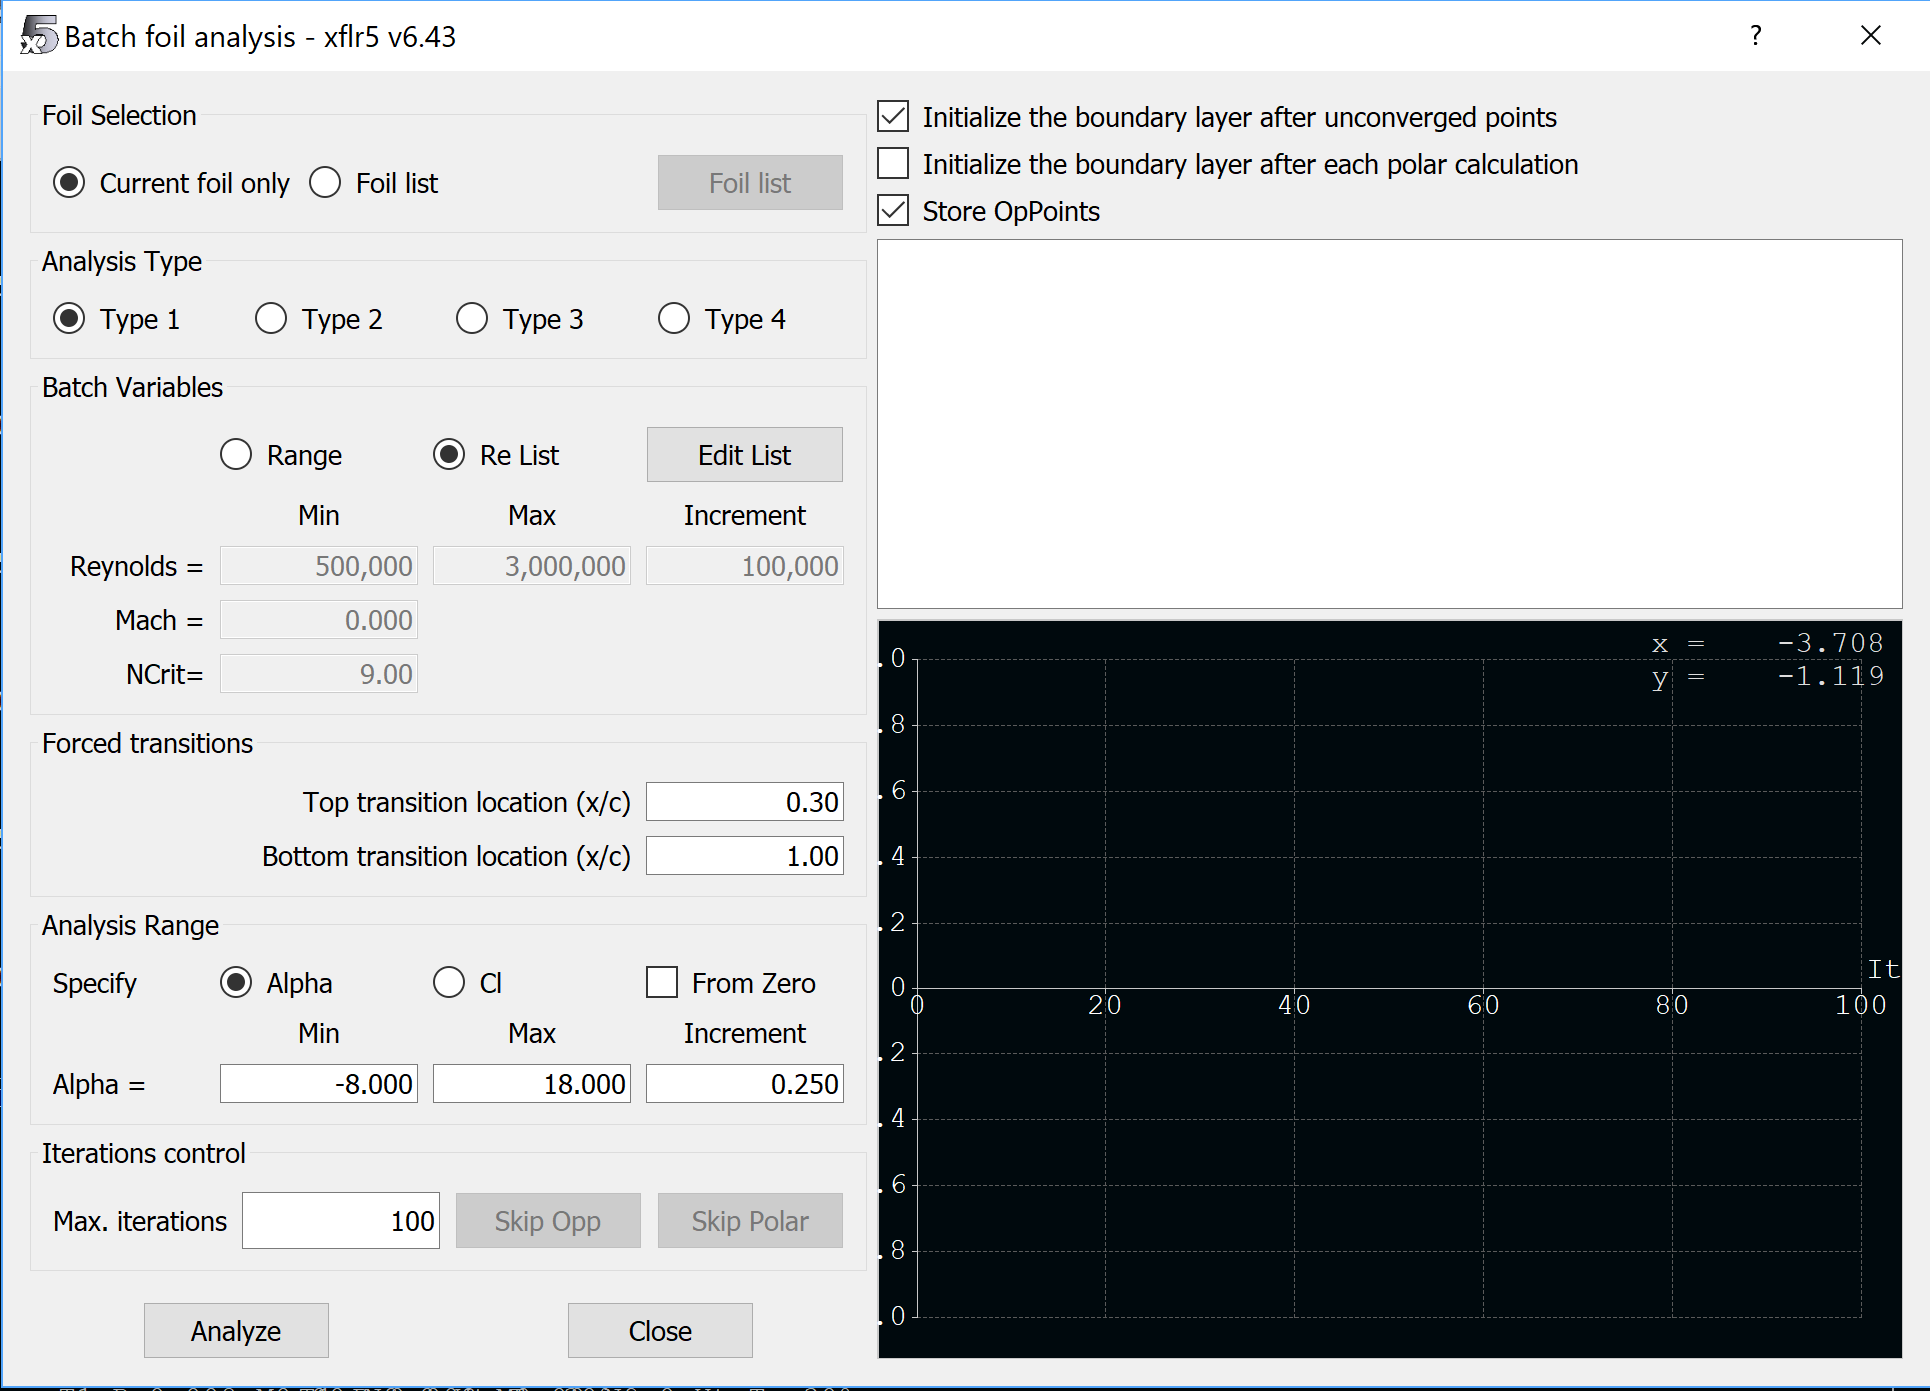
\includegraphics[width=0.95\textwidth]{./figs/airfoilAnalysisSettings.png}
	\captionof{figure}{Dialog window for performing an airfoil batch analysis.}
	\label{settings}
\end{center}

\subsubsection{Plane Analysis}
Next, an analysis was defined for the plane as follows. Bold-faced headings correspond to different tabs in the dialog window when an analysis is defined.

\textbf{Polar Type}
\begin{itemize}
	\item Type 2 (Fixed Lift)
	\item No sideslip ($\beta=0$)
\end{itemize}

\textbf{Analysis}
\begin{itemize}
	\item Horseshoe vortex (VLM1) (No sideslip)
	\item Viscous: YES
	\item Tilt. Geom.: NO
\end{itemize}

\textbf{Inertia}
\begin{itemize}
	\item Use plane inertia: YES
\end{itemize}

\textbf{Ref. dimensions}
\begin{itemize}
	\item Wing Planform projected on xy plane
\end{itemize}

\textbf{Aero data}
\begin{itemize}
	\item $\rho = 1.225 kg/m3$
	\item $\nu = 1.5e-05 m^2/s$
	\item Ground Effect: NO
\end{itemize}

\textbf{Extra Drag}
\begin{itemize}
	\item Extra area($m^2$): 0.05
	\item Extra drag coef.: 0.5*
\end{itemize}

*Note that the drag was roughly approximated as a sphere, with $C_D=0.5$.

\textbf{Analysis settings}
\begin{itemize}
	\item Sequence: YES
	\item Start $=-5.000^\circ$
	\item End $=15.000^\circ$
\end{itemize}

\subsubsection{Stability Analysis}
Next, an analysis was defined for the plane as follows. Bold-faced headings correspond to different tabs in the dialog window when a stability analysis is defined.

\textbf{Analysis}
\begin{itemize}
	\item Plane analysis methods: Mix 3D Panels/VLM2
	\item Viscous Analysis: YES
	\item $\beta = 0.00^\circ$
	\item $\phi = 0.00^\circ$
\end{itemize}

\textbf{Ref. dimensions}
\begin{itemize}
	\item Wing Planform projected on xy plane
\end{itemize}

\textbf{Mass and inertia}
\begin{itemize}
	\item Use plane inertia: YES
\end{itemize}

\textbf{Control parameters}
\begin{itemize}
	\item ALL ZERO
\end{itemize}

\textbf{Aero data}
\begin{itemize}
	\item $\rho = 1.225 kg/m3$
	\item $\nu = 1.5e-05 m^2/s$
	\item Ground Effect: NO
\end{itemize}

\textbf{Extra Drag}
\begin{itemize}
	\item Extra area($m^2$): 0.05
	\item Extra drag coef.: 0.5*
\end{itemize}

\textbf{Analysis settings}
\begin{itemize}
	\item Sequence: NO
\end{itemize}



\section{Results}
The following sections were considered when designing CG placement and design speed.

\subsection{Airfoils}
Drag polars for the airfoil of the main wing at design speed conditions are included in Fig. \ref{airfoilPolars}. The  design speed condition was selected as $12m/s$ with a Reynold's number of $224,000$ (based on $\nu=1.5e-5$ and a mean aerodynamic chord of $\textnormal{mac}=0.28~m$). Since the linear regime of the $c_l vs. \alpha$ plot ends at approximately $9.2^\circ$ and reaches a maximum at approximately $13^\circ$. Since we have about $5^\circ$ of wash-in in the wing design, it is desirable to fly at an angle of attack of $\alpha < 13^\circ - 5^\circ = 8^\circ$ to avoid tip stall. However, even some tip stall should not be catastrophic as the ailerons lie completely in a 0-twist section of the wing.

\begin{center}
	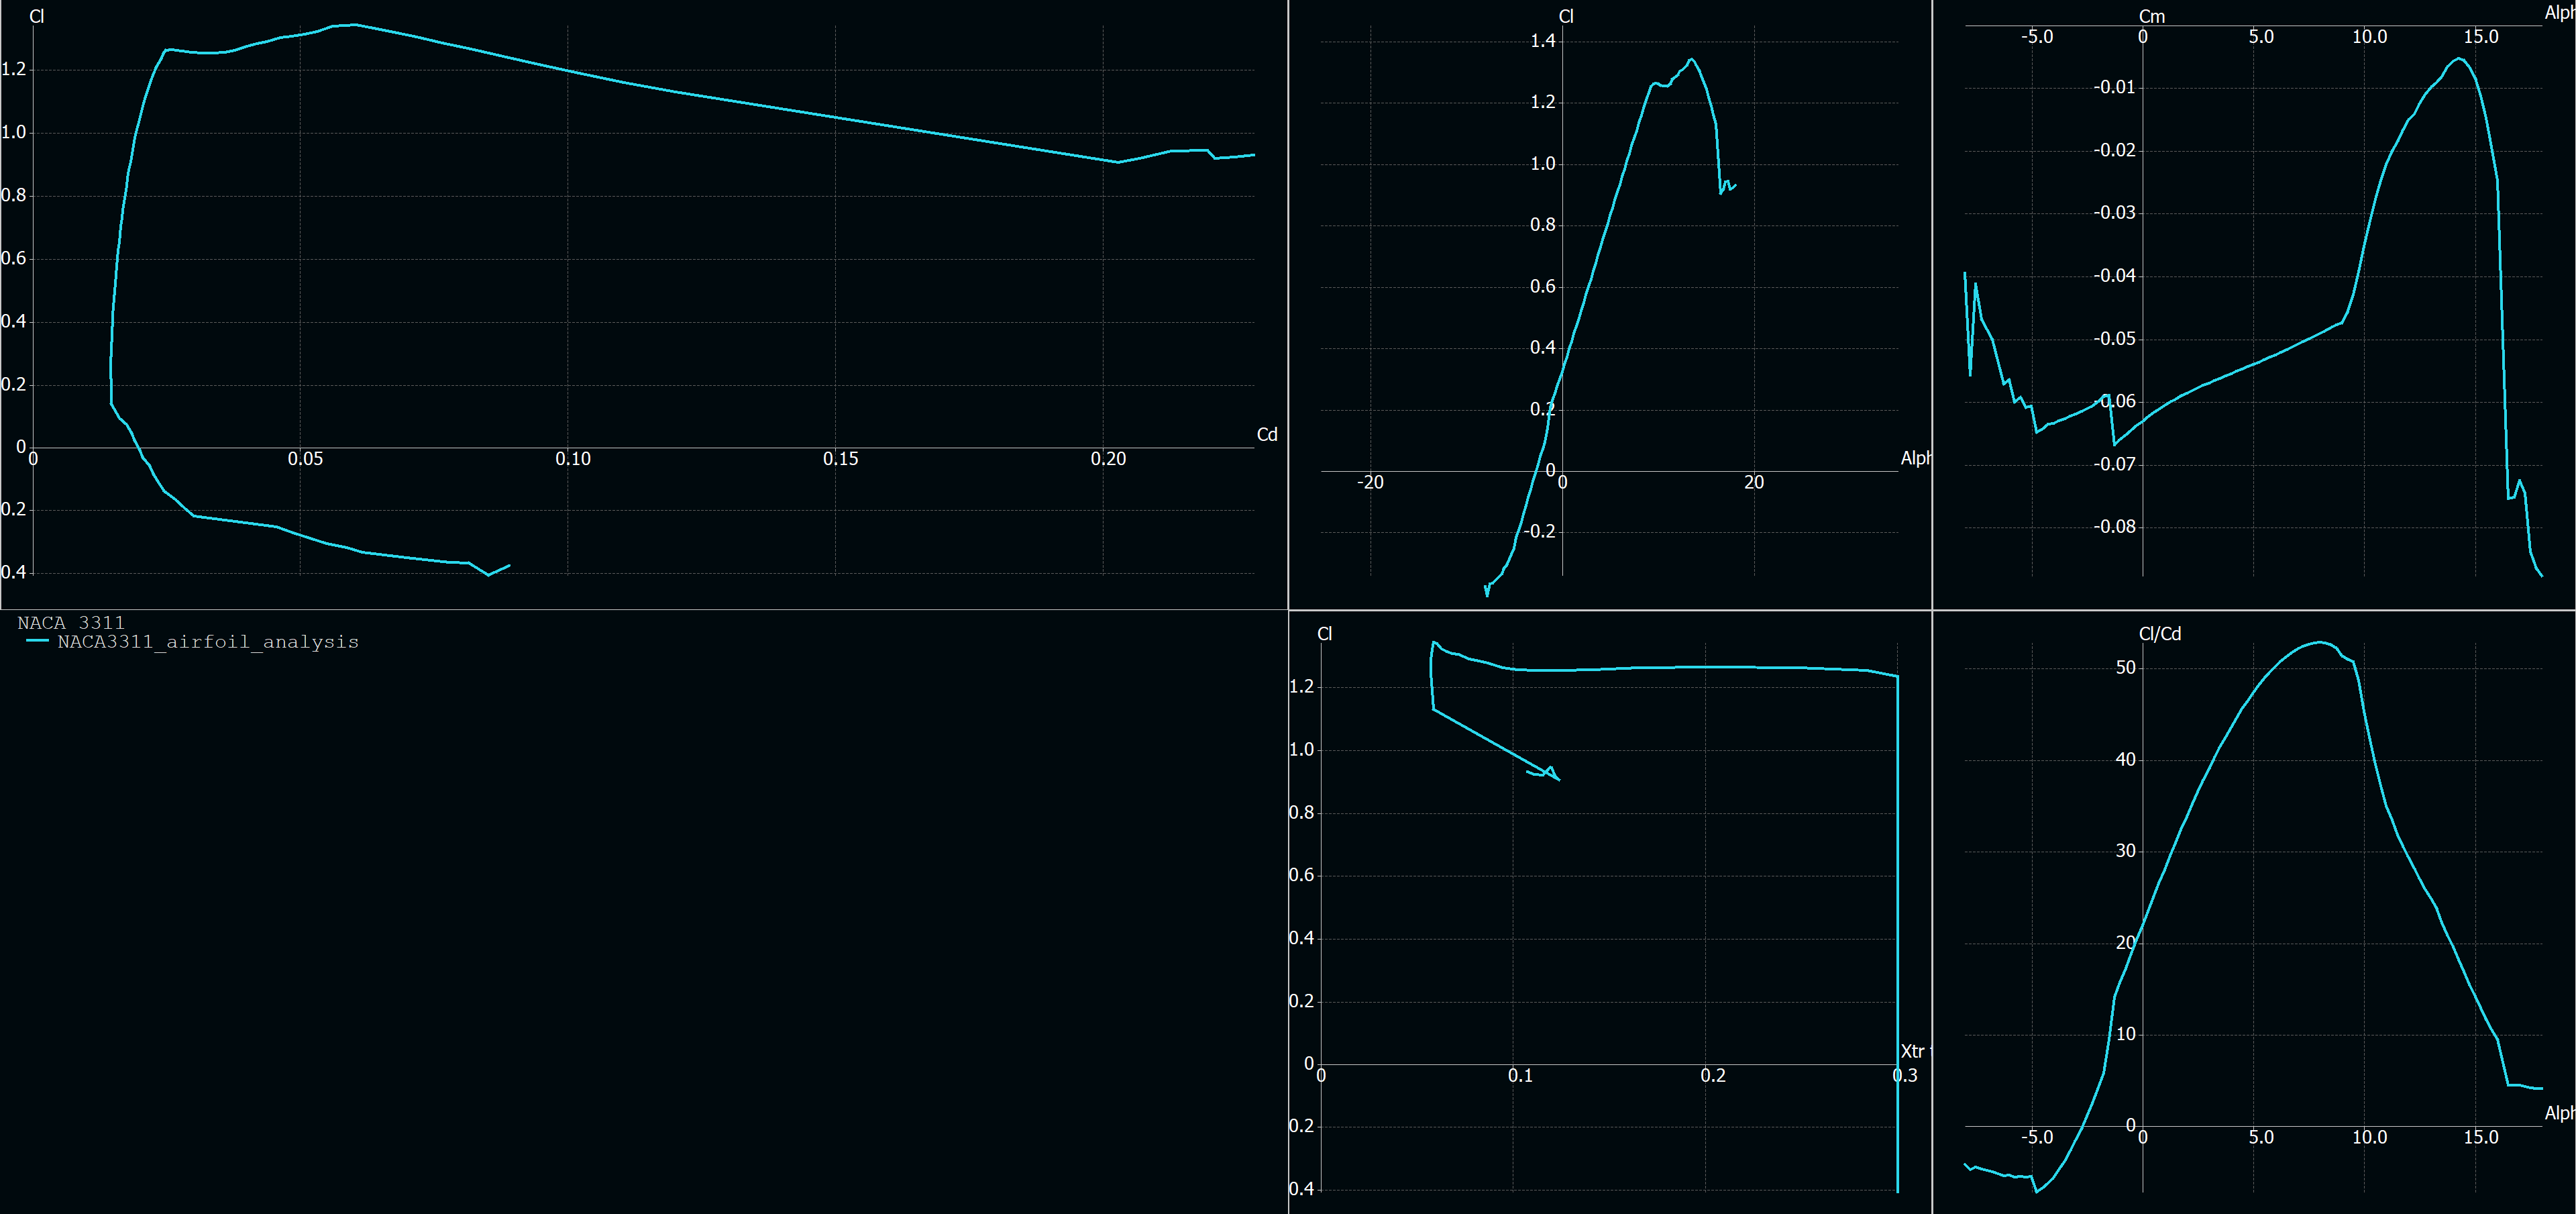
\includegraphics[width=0.80\textwidth]{./figs/Polars20190116.png}
	\captionof{figure}{Drag polars of the main wing airfoil at design speed conditions.}
	\label{airfoilPolars}
\end{center}

\subsection{Plane Analysis}

A rendering of the analyzed plane is included in Fig. \ref{rendering}, with drag polars included in Fig. \ref{planePolars}. It is clear from the $C_L$ vs. $V$ plot that a lower flight speed corresponds to a higher lift coefficient, with diminishing returns. The lift coefficient varies quite linearly with angle of attack, as shown in the $C_L$ vs. $\alpha$ plot. The goal, then, is to increase the design angle of attack as much as possible without running the danger of tip stall. Serendipitously, this has the effect of increasing the lift-to-drag ratio, as seen in the $C_L/C_D$ vs. $\alpha$ plot. This will correspond to an increase in range and endurance, both of which are desirable for increasing flight time on a single battery during testing and in the competition. A target design angle of attack of $7^\circ$ was selected, about $1^\circ$ away from the tip stall condition discussed in the previous section. Again, since the ailerons are not located in the tip-stall region, we felt comfortable with the small safety factor this entails.

In order to change the design angle of attack, the center of gravity and tail incidence angle were adjusted. The tail incidence angle of the Nimbus Pro is zero off the shelf, requiring significant elevator deflection for steady level flight, increasing required trim and therefore drag. Further, the XFLR5 analysis could not be performed because control surfaces were not modeled. In order to mitigate this, the tail incidence angle was adjusted in simulation. After placing the CG at an initial guess, the tail angle was increased until a reasonably negative $C_{m,\alpha}$ (slope of the $Cm$ vs. $\alpha$ plot) was obtained. Because the $Cm$ vs. $\alpha$ plot also depends on the CG, tail incidence angle and CG were adjusted iteratively. Fig. \ref{tailIncidence} shows the drag polars resulting from 5 adjustments of the tail incidence angle as well as its . The effect of the tail incidence angle is most apparent in the $C_{m,\alpha}$ plot (upper right). Note that the bottom-most white curve represents the performance of the plane with its $0^\circ$ out-of-the-box tail incidence. This is unacceptable without trim, as it would fly at a negative angle of attack, resulting in a near-zero lift coefficient, and a probable crash. Contrast this with the blue curve of the $C_{m,\alpha}$ plot, which would result in a statically stable flight at an angle of attack of our target $7^\circ$.

Next, the center of gravity location was considered. Since steady level flight occurs when the sum of longitudinal pitching moments equals 0, or $C_m = 0$ on the $C_m$ vs. $\alpha$ plot, adjusting the lever arm of the plane's weight has a strong influence on the stable angle of attack. After iterating on the CG location in the plane and tail incidence angle to maximize the lift-to-drag ratio (shown on the $C_L$ vs. $C_D$ plot) and minimize design velocity (shown on the $C_L$ vs. $V$ plot), it was determined that a CG placement of 6.2~cm in front of the leading edge of the wing results is the optimal condition. The resulting tail incidence angle was $7.5^\circ$. This resulted in a design angle of attack of about $7^\circ$, consistent with our target value. We calculated a static margin of about 5\%. Though slightly low, the plane was still stable, and we believed that the increased aerodynamic performance to be worth the small static margin. Also of note, plans were subsequently made to modify the tail incidence angle to $7.5^\circ$. See AF-10 for the tail modification design artifact.

\begin{center}
	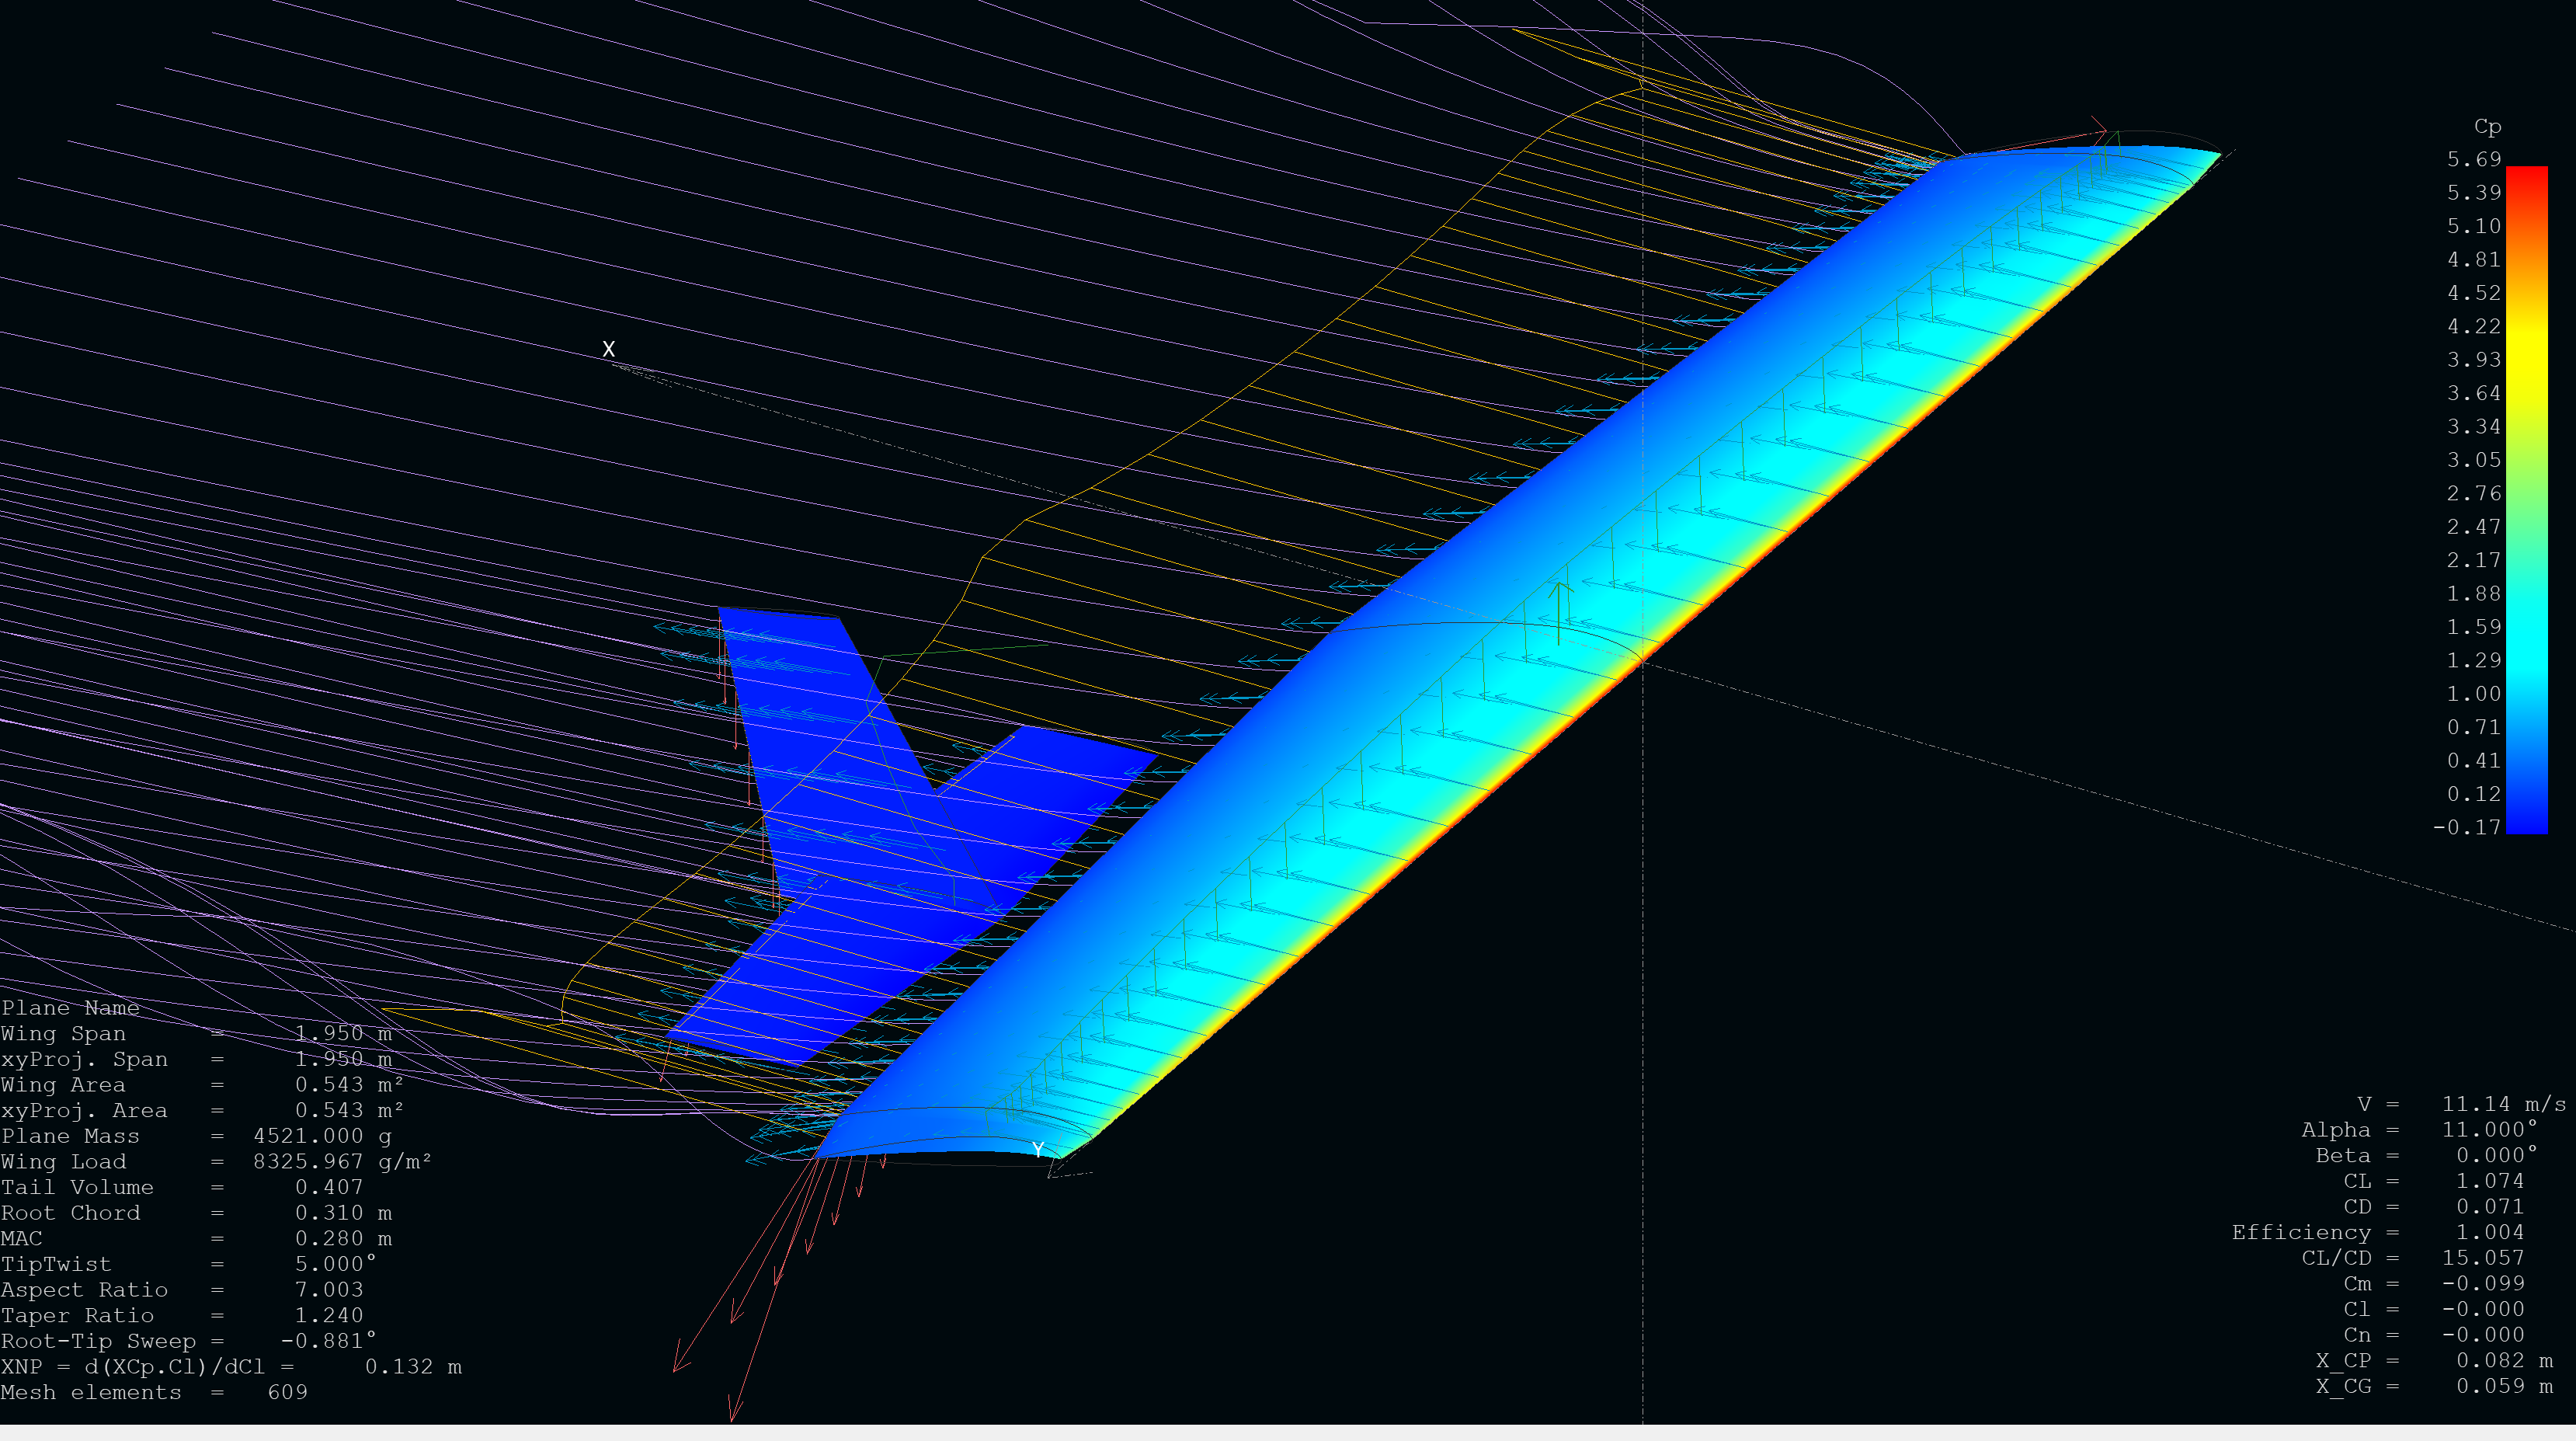
\includegraphics[width=0.80\textwidth]{./figs/awesomeMeaninglessRendering.png}
	\captionof{figure}{Rendering of the analyzed plane.}
	\label{rendering}
\end{center}

\begin{center}
	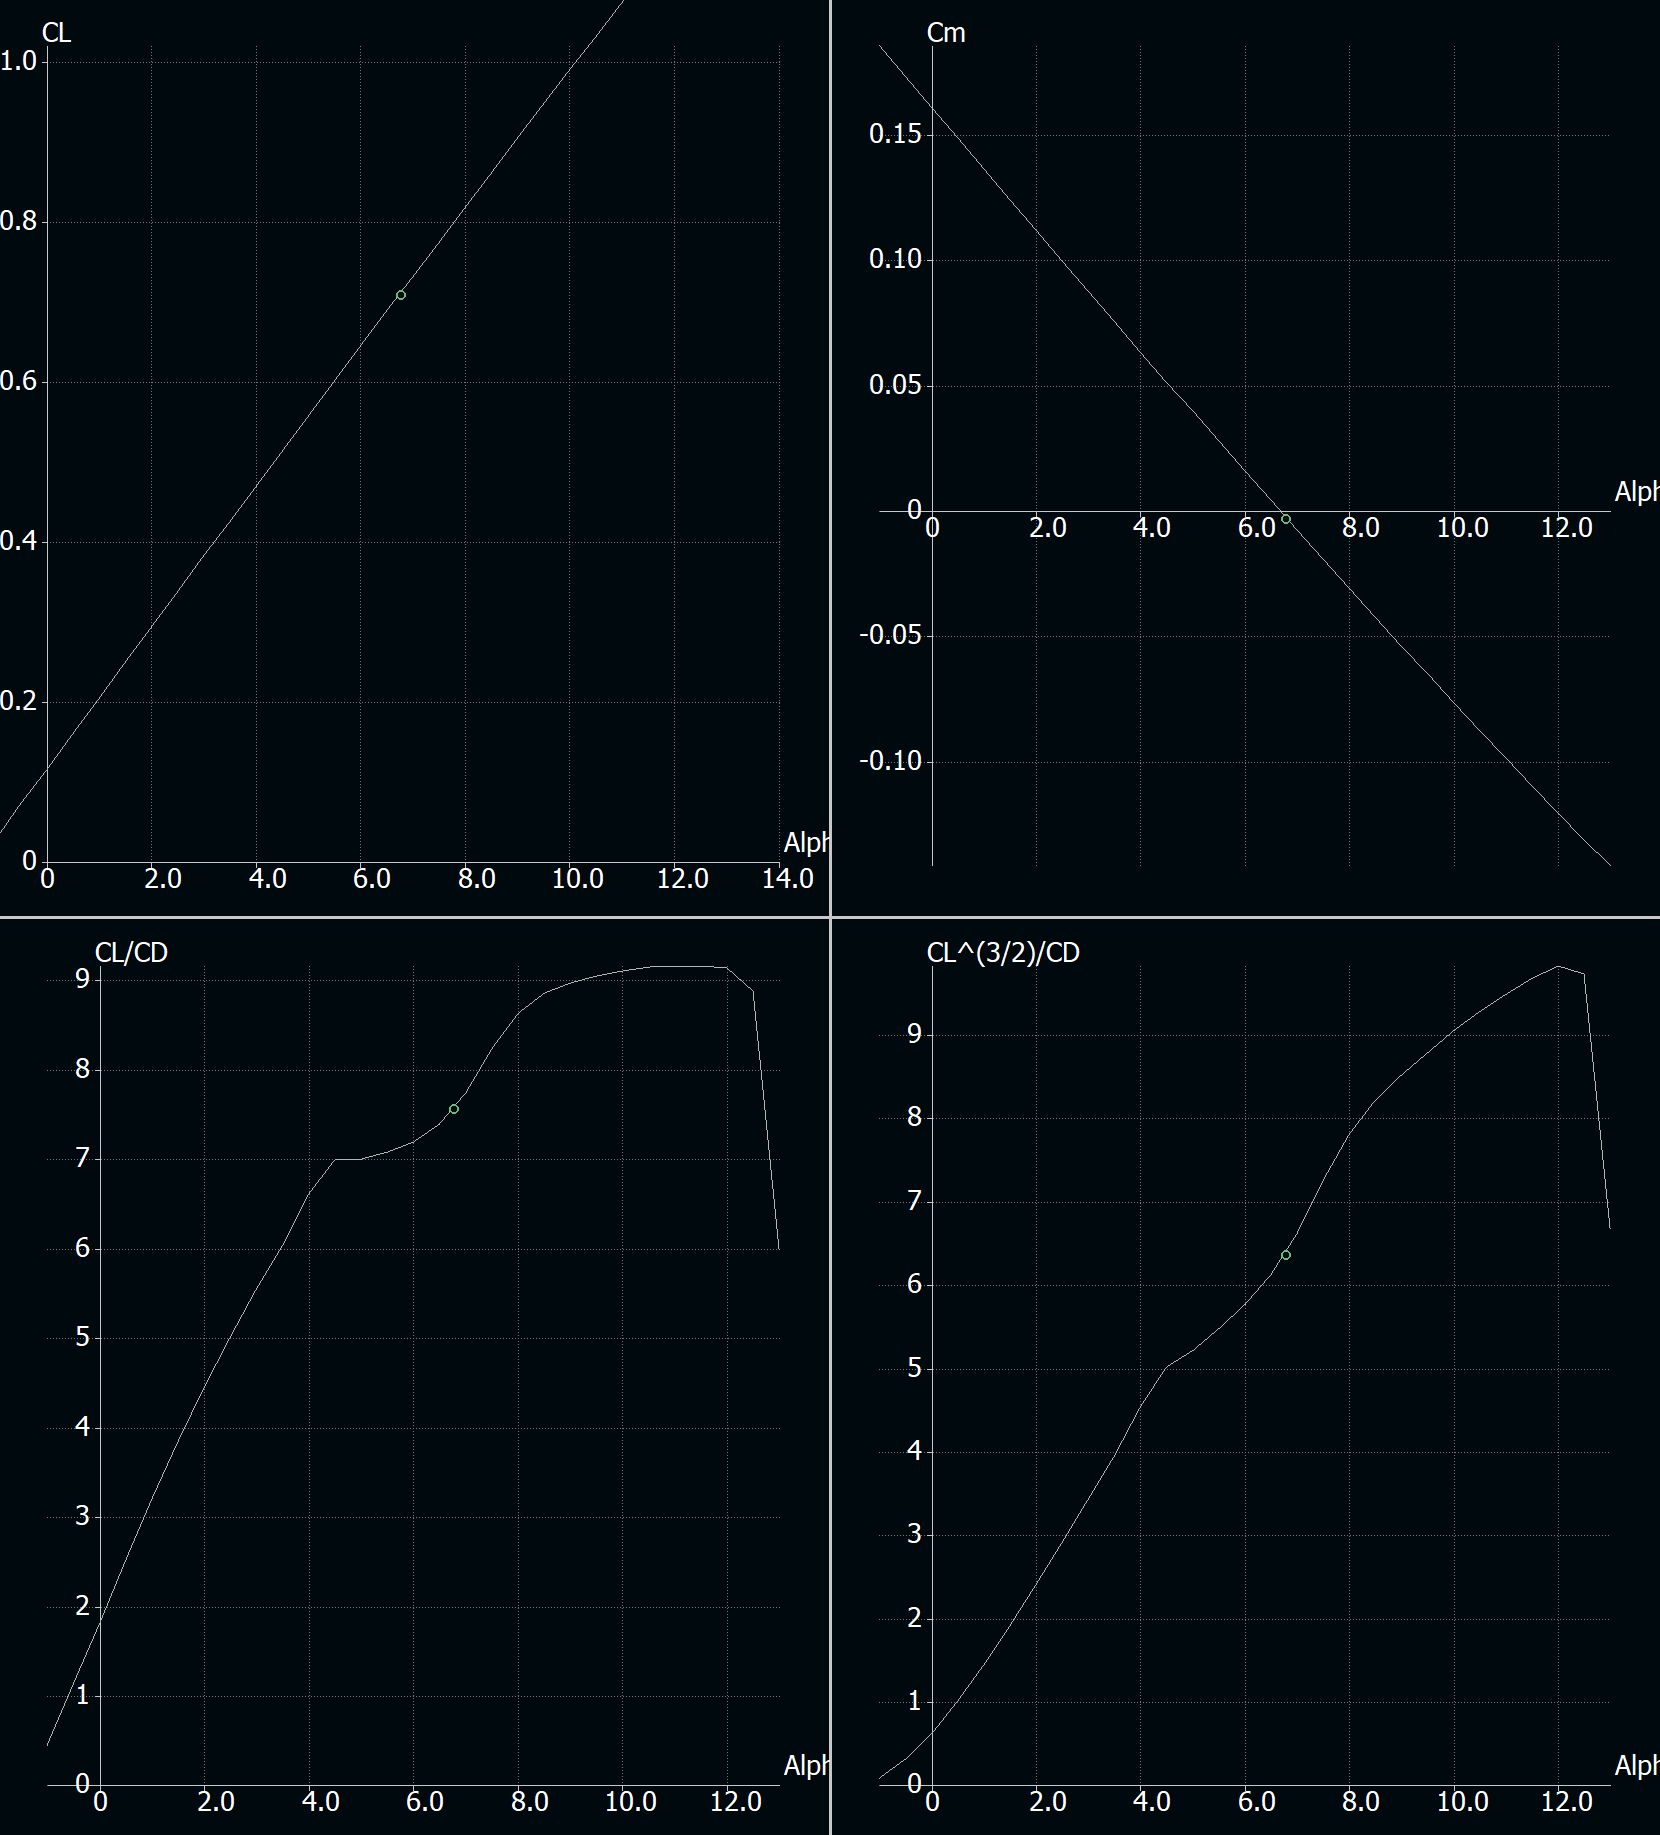
\includegraphics[width=0.70\textwidth]{./figs/LiftDragPolars.png}
	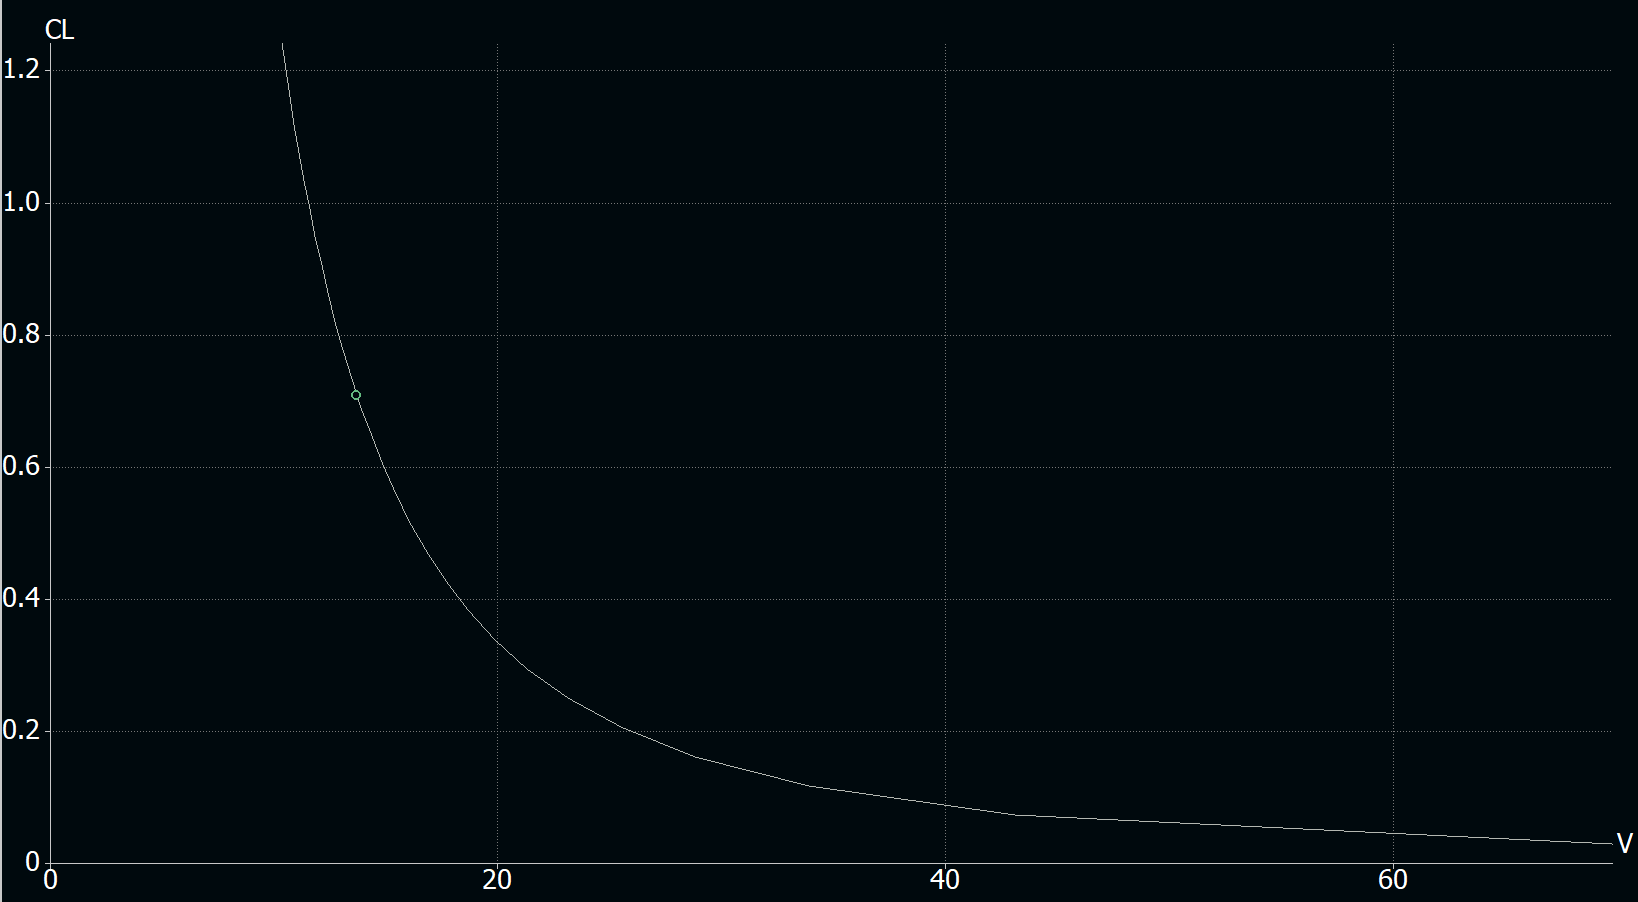
\includegraphics[width=0.70\textwidth]{./figs/CLvV.png}
	\captionof{figure}{Drag polars of the plane.}
	\label{planePolars}
\end{center}

\subsection{Stability Analysis}
For increased image clarity and easier waypoint navigation, a statically and dynamically stable airframe is desired.
\subsubsection{Static Stability}
The results of the static stability analysis are included in Fig. \ref{static}. Of note:
\begin{itemize}
	\item $Cnb > 0$ indicating static directional stability (yaw axis).
	\item $Cma<0$ indicating static longitudinal stability (pitch axis).
	\item $Clb>0$ indicating slight static roll instability.
\end{itemize}

While the roll instability is alarming at first, it is very slight and was believed to be easily overcome by the R/C pilot or the flight controller as needed. Extensive field testing proved the plane to be nearly neutrally roll stable, meaning the plane maintains a constant roll state until ailerons are activated. It is possible that deflection of the foam wings during flight produces a slight dihedral that overcomes any roll instability. the plane may have.

\begin{center}
	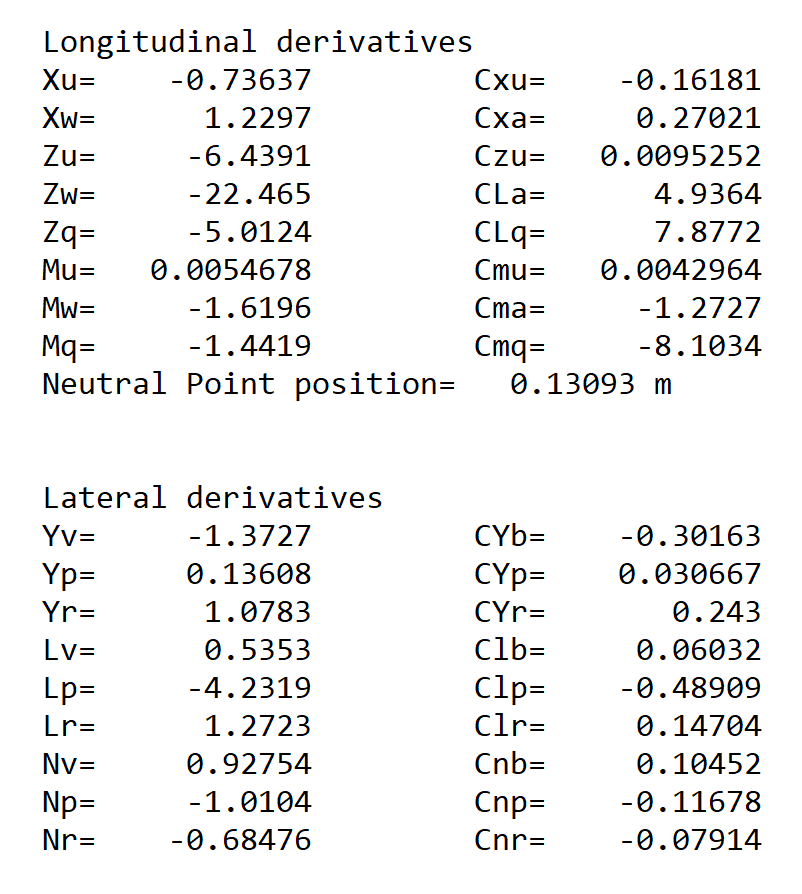
\includegraphics[width=0.50\textwidth]{./figs/staticStability.png}
	\captionof{figure}{Tabulated static stability derivatives.}
	\label{static}
\end{center}

\subsection{Dynamic Stability}

The dynamic stability analysis (included in Fig. \ref{dynamic} ) reveals negative real parts for all stability eigenvalues except for spiral stability, indicating a stable plane for all but that mode. The severity of this instability was investigated by animating the plane. The "Lateral" radio button was selected and the fourth mode selected in the stability dialog window. The timeframe required for the plane to deflect a single wingspan was nearly 10 seconds; this is ample time for a course correction to be made either by the R/C pilot or the flight controller, and the spiral instability was determined to be negligible.

\begin{center}
	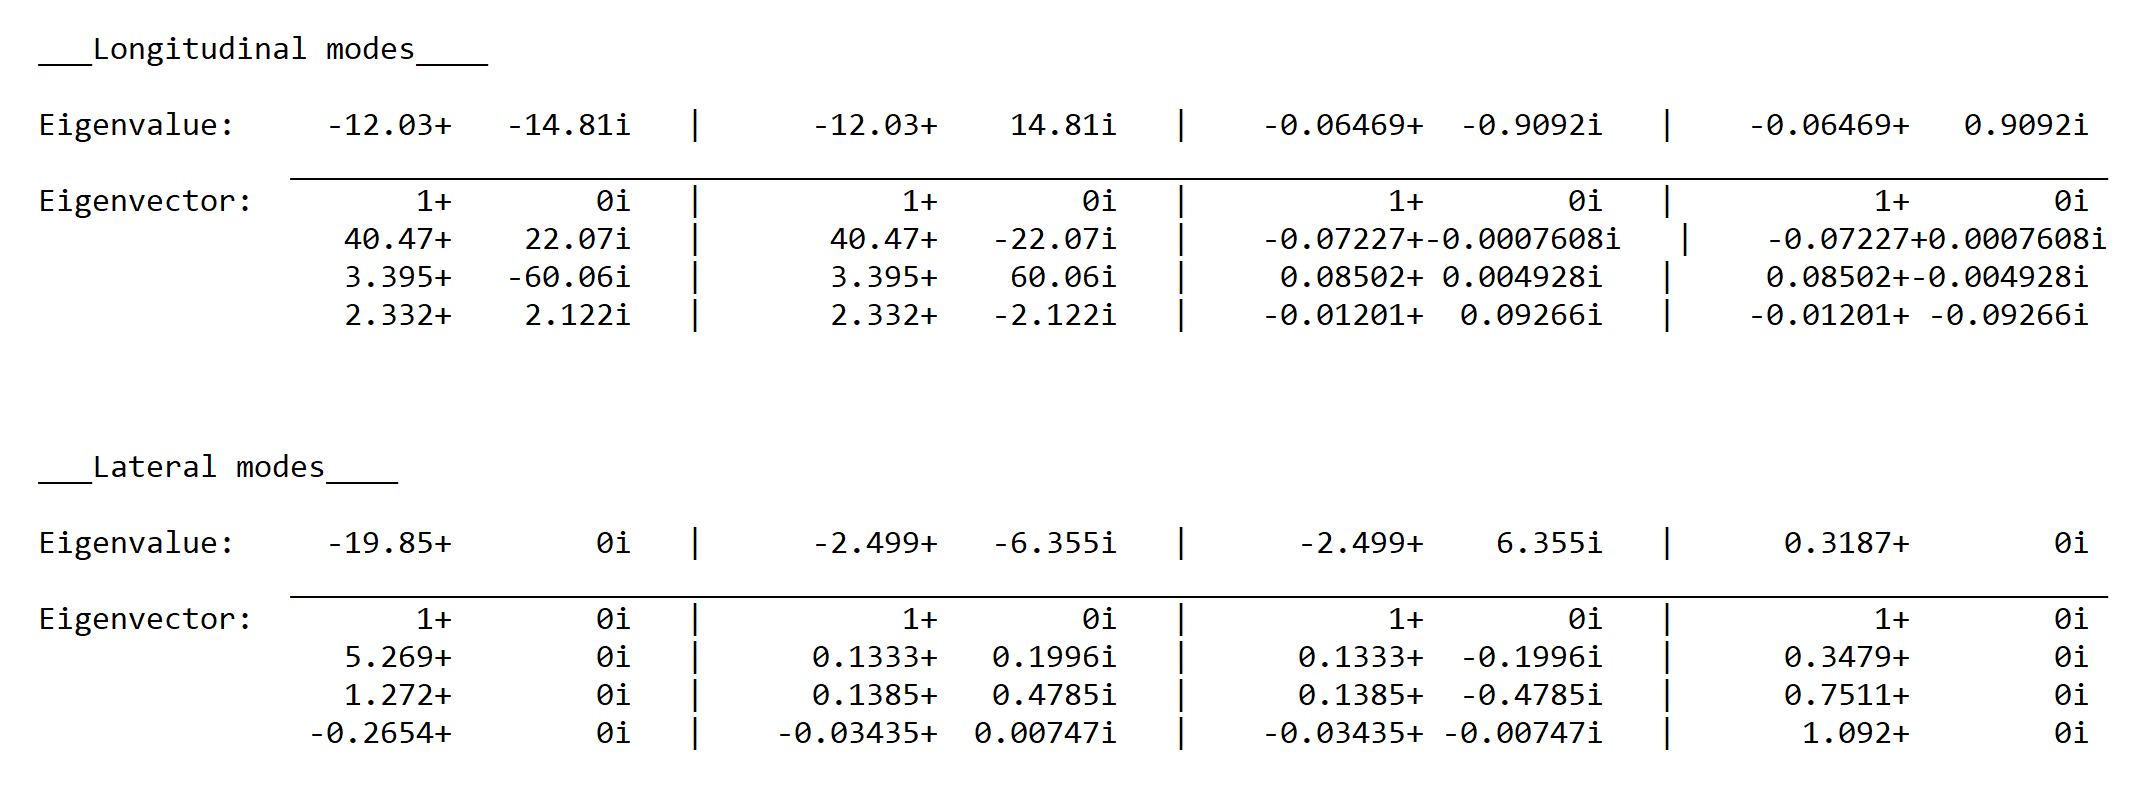
\includegraphics[width=0.95\textwidth]{./figs/dynamicStability.png}
	\captionof{figure}{Tabulated dynamic stability eigenvalues.}
	\label{dynamic}
\end{center}

\section{Conclusion}

In summary, the aerodynamic performance of the aircraft was modeled and optimized using the XFLR5 open-source software. The following key results were achieved:

\begin{itemize}
	\item It was determined that the tail incidence angle should be increased to $7.5^\circ$ to significantly reduce elevator trim.
	\item It was determined that the center of gravity should be placed at 6.2~cm from the leading edge of the wing to optimize aerodynamic performance.
	\item Design speed was decreased from about 20~m/s to 13~m/s: a 35\% decrease from last year.
	\item The design tested sufficiently stable in all modes, static and dynamic.
\end{itemize}

These test results have provided invaluable direction and insight into the design of this year's airframe.


\end{document}
